\documentclass[12 pt]{article}
\usepackage[utf8]{inputenc}
\usepackage{matlab-prettifier}
\usepackage[portuguese]{babel}
\usepackage{indentfirst}
\usepackage{graphicx}
\usepackage{float}
\usepackage{subcaption}
\usepackage[font=small,labelfont=bf]{caption}
\definecolor{mygreen}{RGB}{28,172,0} % color values Red, Green, Blue
\definecolor{myyellow}{rgb}{1.0, 1.0, 0.8}
\usepackage{mathtools}
\usepackage{multirow}
\usepackage{comment}
\usepackage{xcolor}
\usepackage{colortbl}
\usepackage[normalem]{ulem}               % to striketrhourhg text
\usepackage{amsmath}
\usepackage{amsfonts}
\usepackage{hyperref}
\usepackage{tcolorbox}
\usepackage{longtable}
\usepackage{enumitem}
\newcommand\redout{\bgroup\markoverwith
{\textcolor{red}{\rule[0.5ex]{2pt}{0.8pt}}}\ULon}
\renewcommand{\lstlistingname}{Código}% Listing -> Algorithm
\renewcommand{\lstlistlistingname}{Lista de \lstlistingname s}% List of Listings -> List of Algorithms

\usepackage[top=3cm,left=2cm,bottom=2cm, right=2cm]{geometry}
\usepackage{tikz}
\usetikzlibrary{decorations.pathreplacing}
\usetikzlibrary{automata}
\usetikzlibrary{positioning}
\usetikzlibrary{arrows.meta, positioning}

\usepackage{adjustbox}


% Configuração para destacar a sintaxe do Python
\lstset{ 
    language=Python,                     % A linguagem do código
    backgroundcolor=\color{myyellow}, % A cor do fundo 
    basicstyle=\ttfamily\footnotesize,   % O estilo do texto básico
    keywordstyle=\color{blue},           % Cor das palavras-chave
    stringstyle=\color{red},             % Cor das strings
    commentstyle=\color{mygreen},          % Cor dos comentários
    numbers=left,                        % Números das linhas à esquerda
    numberstyle=\tiny\color{gray},       % Estilo dos números das linhas
    stepnumber=1,                        % Número de linhas entre os números das linhas
    frame=single,                        % Moldura ao redor do código
    breaklines=true,                     % Quebra automática das linhas longas
    captionpos=t,                        % Posição da legenda
    showstringspaces=false               % Não mostra espaços em branco nas strings
    extendedchars=true,
    literate={º}{{${ }^{\underline{o}}$}}1 {á}{{\'a}}1 {à}{{\`a}}1 {ã}{{\~a}}1 {é}{{\'e}}1 {É}{{\'E}}1 {ê}{{\^e}}1 {ë}{{\"e}}1 {í}{{\'i}}1 {ç}{{\c{c}}}1 {Ç}{{\c{C}}}1 {õ}{{\~o}}1 {ó}{{\'o}}1 {ô}{{\^o}}1 {ú}{{\'u}}1 {â}{{\^a}}1 {~}{{$\sim$}}1
}


\title{%
\textbf{\huge Universidade Federal do Rio de Janeiro} \par
\textbf{\LARGE Instituto Alberto Luiz Coimbra de Pós-Graduação e Pesquisa de Engenharia} \par


\includegraphics[width=8cm]{COPPE UFRJ.png} \par

\textbf{Programa de Engenharia de Sistemas e Computação} \par

COS868 - Probabilidade e Estatística para Aprendizado de Máquina \par

Profa. Dra. Rosa M. Leão (PESC/COPPE/UFRJ)\par

\vspace{1\baselineskip}
\textbf{\textit{Projeto do Curso}} \par
}

\author{Luiz Henrique Souza Caldas\\email: lhscaldas@cos.ufrj.br}

\date{\today}

\begin{document}
\maketitle

\tableofcontents

\section{Introdução}

\subsection{Objetivo}

O objetivo deste trabalho é realizar uma análise de um conjunto de dados reais fornecidos por um provedor de Internet de médio porte, avaliando as taxas de upload e download de dispositivos domésticos, especificamente Smart-TVs e Chromecasts, com base na teoria aprendida em classe, destacando a importância de uma análise crítica dos resultados obtidos.

\subsection{Análise Exploratória dos Dados}\label{sec:eda}

A análise exploratória foi realizada para compreender as características principais dos dados obtidos dos dispositivos Smart TV e Chromecast. Os resultados estão detalhados abaixo:

\begin{itemize}
    \item \textbf{Primeiras linhas dos dados:}
    \begin{itemize}
        \item \textbf{Smart TV:}
        \begin{verbatim}
            device_id            date_hour       bytes_up    bytes_down
        0   77209603  2021-11-22 15:23:00  132932.983607  2.818140e+06
        1   77209603  2021-11-22 15:24:00  115770.491803  2.264410e+06
        2   77209603  2021-11-22 15:25:00  114030.032787  2.309270e+06
        3   77209603  2021-11-22 15:26:00   97170.622951  2.006544e+06
        4   77209603  2021-11-22 15:27:00   39569.573770  8.061440e+05
        \end{verbatim}
        
        \item \textbf{Chromecast:}
        \begin{verbatim}
            device_id            date_hour     bytes_up    bytes_down
        0   66161985  2021-09-06 00:01:00  2987.016393  49185.704918
        1   66161985  2021-09-06 00:02:00   685.935484    328.258065
        2   66161985  2021-09-06 00:03:00  4493.901639  37914.064516
        3   66161985  2021-09-06 00:04:00   776.133333    229.200000
        4   66161985  2021-09-06 00:05:00  3081.311475  51656.800000
        \end{verbatim}
    \end{itemize}
    
    \item \textbf{Dimensões dos dados:}
    \begin{itemize}
        \item Smart TV: (4417903, 4)
        \item Chromecast: (1620529, 4)
    \end{itemize}

    \item \textbf{Dados faltantes:}
    \begin{itemize}
        \item Smart TV: Nenhum valor faltante em \texttt{device\_id}, \texttt{date\_hour}, \texttt{bytes\_up}, \texttt{bytes\_down}.
        \item Chromecast: Nenhum valor faltante em \texttt{device\_id}, \texttt{date\_hour}, \texttt{bytes\_up}, \texttt{bytes\_down}.
    \end{itemize}

    \item \textbf{Valores zero:}
    \begin{itemize}
        \item Smart TV: \texttt{bytes\_up} = 1.803.853, \texttt{bytes\_down} = 1.978.337.
        \item Chromecast: \texttt{bytes\_up} = 6.057, \texttt{bytes\_down} = 4.099.
    \end{itemize}

    \item \textbf{Valores negativos:}
    \begin{itemize}
        \item Smart TV: Nenhum valor negativo em \texttt{bytes\_up} ou \texttt{bytes\_down}.
        \item Chromecast: Nenhum valor negativo em \texttt{bytes\_up} ou \texttt{bytes\_down}.
    \end{itemize}
\end{itemize}


\subsection{Pré-processamento}

O pré-processamento foi realizado para preparar os dados dos dispositivos Smart TV e Chromecast para análises posteriores. As etapas realizadas são descritas a seguir:

\begin{itemize}
    \item \textbf{Carregamento dos dados:} Os dados foram lidos a partir dos arquivos \texttt{dataset\_smart-tv.csv} e \texttt{dataset\_chromecast.csv}.

    \item \textbf{Correção de valores zero:} Como as colunas \texttt{bytes\_up} e \texttt{bytes\_down} apresentavam valores zero, foi aplicado um \textit{shift} de +1 a todos os valores dessas colunas para evitar problemas no cálculo do logaritmo.

    \item \textbf{Reescalonamento dos dados:} Os valores das colunas \texttt{bytes\_up} e \texttt{bytes\_down} foram transformados para a escala logarítmica na base 10 (\texttt{log10}), devido à grande variação na ordem de grandeza desses valores.

    \item \textbf{Ordenação temporal:} Os dados foram ordenados pela coluna \texttt{date\_hour} para garantir a consistência temporal nas análises subsequentes.

    \item \textbf{Salvamento dos dados processados:} Os datasets resultantes podem ser salvos como arquivos CSV (\texttt{smart\_preprocessado.csv} e \texttt{chrome\_preprocessado.csv}) para uso posterior.
\end{itemize}

Essa etapa garante que os dados estejam limpos, reescalonados e organizados, facilitando análises estatísticas e a geração de gráficos. Além disso, a transformação logarítmica reduz a influência de valores extremos, melhorando a interpretação dos resultados. 

\section{Estatísticas Gerais}

Nesta seção, são apresentadas as estatísticas gerais dos dados coletados para os dispositivos \textit{Smart-TV} e \textit{Chromecast}. As análises incluem cálculos de medidas descritivas, como média, variância e desvio padrão, além de representações gráficas através de histogramas, boxplots e funções de distribuição empírica (ECDF). 

\subsection{Medidas Descritivas}

As medidas descritivas para as taxas de \textit{upload} e \textit{download} (em escala logarítmica base 10) estão resumidas na Tabela~\ref{tab:estatisticas}. 

\begin{table}[H]
\centering
\caption{Medidas descritivas das taxas de \textit{upload} e \textit{download}.}
\label{tab:estatisticas}
\begin{tabular}{|c|c|c|c|c|}
\hline
\textbf{Dispositivo} & \textbf{Tipo de Tráfego} & \textbf{Média} & \textbf{Variância} & \textbf{Desvio Padrão} \\ \hline
\textit{Smart-TV} & \textit{Upload} & 2.16 & 4.11 & 2.03 \\ \hline
\textit{Smart-TV} & \textit{Download} & 2.35 & 6.72 & 2.59 \\ \hline
\textit{Chromecast} & \textit{Upload} & 3.35 & 0.46 & 0.68 \\ \hline
\textit{Chromecast} & \textit{Download} & 3.80 & 1.66 & 1.29 \\ \hline
\end{tabular}
\end{table}

\subsection{Visualizações Gráficas}

Para compreender melhor a distribuição dos dados, são utilizadas as seguintes representações gráficas:

\begin{itemize}
    \item \textbf{Histogramas:} As distribuições das taxas de \textit{upload} e \textit{download} para cada dispositivo estão representadas nos histogramas da Figura~\ref{fig:histogramas}.
    \item \textbf{Boxplots:} A Figura~\ref{fig:boxplots} mostra os boxplots comparando as taxas de \textit{upload} e \textit{download} entre \textit{Smart-TV} e \textit{Chromecast}.
    \item \textbf{ECDF:} As funções de distribuição empírica, exibidas na Figura~\ref{fig:ecdf}, demonstram a probabilidade acumulada para cada valor das taxas.
\end{itemize}

Para a construção dos histogramas, o número de bins foi calculado utilizando o método de Sturges:

\begin{equation}\label{eq:sturges}
k = 1 + \log_2(n),
\end{equation}

onde \(n\) é o número total de amostras. Este método busca otimizar a visualização dos dados ao balancear granularidade e clareza.

O número de bins calculado para cada dispositivo é o seguinte:
\begin{itemize}
    \item \textbf{\textit{Smart-TV}:} \(k = 24\) bins.
    \item \textbf{\textit{Chromecast}:} \(k = 22\) bins.
\end{itemize}

\begin{figure}[H]
    \centering
    \includegraphics[width=0.8\textwidth]{../estatísticas gerais/histogramas.png}
    \caption{Histogramas das taxas de \textit{upload} e \textit{download} para \textit{Smart-TV} e \textit{Chromecast}.}
    \label{fig:histogramas}
\end{figure}

\begin{figure}[H]
    \centering
    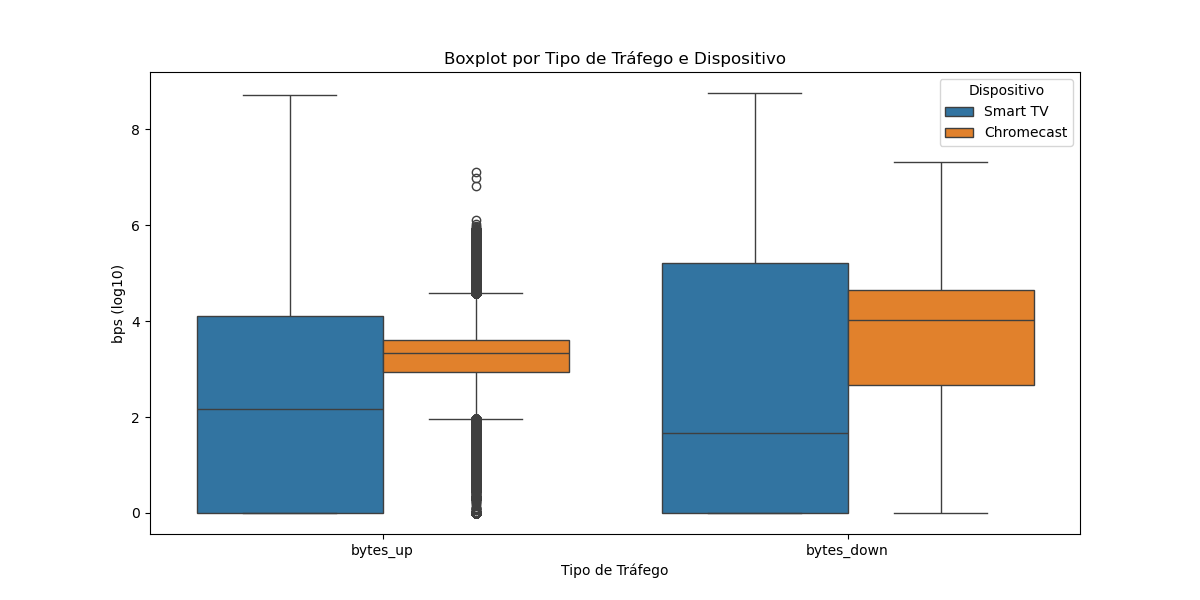
\includegraphics[width=0.8\textwidth]{../estatísticas gerais/boxplot.png}
    \caption{Boxplots das taxas de \textit{upload} e \textit{download} para \textit{Smart-TV} e \textit{Chromecast}.}
    \label{fig:boxplots}
\end{figure}

\begin{figure}[H]
    \centering
    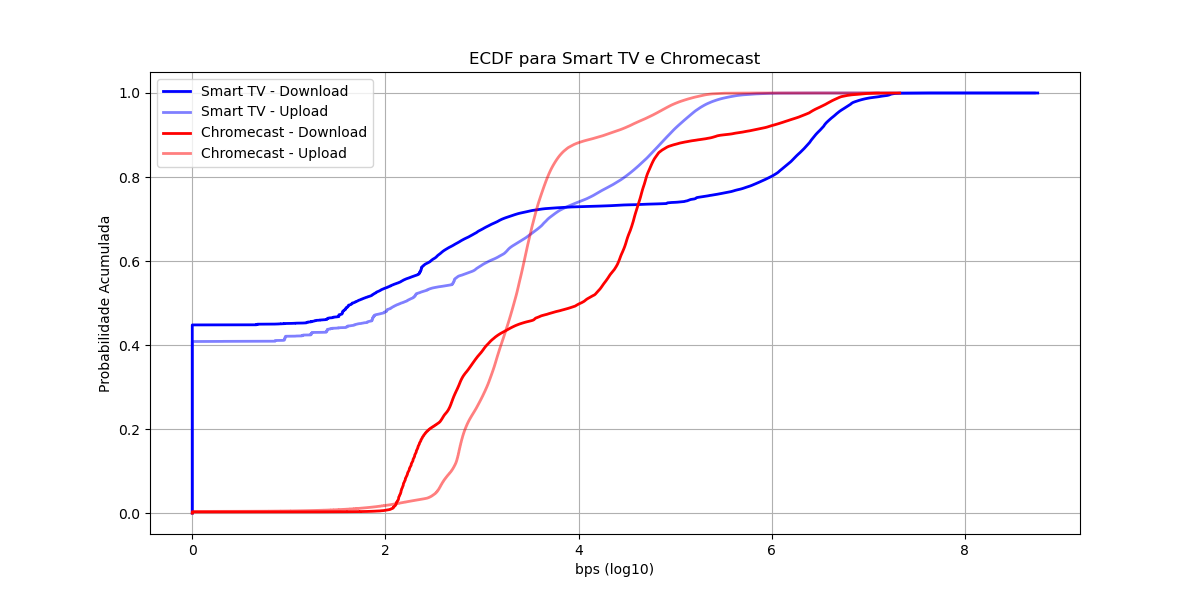
\includegraphics[width=0.8\textwidth]{../estatísticas gerais/ecdf.png}
    \caption{Funções de Distribuição Empírica (ECDF) das taxas de \textit{upload} e \textit{download}.}
    \label{fig:ecdf}
\end{figure}

As visualizações gráficas fornecem informações importantes para o provedor de serviços ao identificar padrões de tráfego específicos de cada dispositivo. Por exemplo, histogramas permitem entender a distribuição predominante de dados, enquanto os boxplots destacam possíveis valores atípicos que podem impactar negativamente a rede. Essas análises auxiliam na definição de prioridades no gerenciamento do tráfego de rede, garantindo uma melhor alocação de recursos para dispositivos com padrões mais variáveis.

\subsection{Análise dos Resultados}

Os resultados destacam diferenças importantes nas características das taxas de \textit{upload} e \textit{download} entre os dispositivos \textit{Smart-TV} e \textit{Chromecast}, com implicações práticas significativas para o provedor de serviços de Internet.

\textbf{\textit{Smart-TV}:} As taxas de \textit{upload} e \textit{download} da \textit{Smart-TV} apresentam médias similares e variâncias relativamente altas, refletindo maior dispersão dos dados. A alta concentração de valores baixos, especialmente iguais a zero, é evidenciada pela primeira barra dominante nos histogramas (Figura~\ref{fig:histogramas}) e pela ECDF inicial, que ultrapassa 0.4 devido aos valores nulos. O boxplot (Figura~\ref{fig:boxplots}) confirma a ausência de outliers, indicando que o tráfego da \textit{Smart-TV} é caracterizado por períodos de inatividade alternados com picos de alta demanda. 

\textbf{\textit{Chromecast}:} O \textit{Chromecast} apresenta padrões diferentes, com taxas de \textit{upload} e \textit{download} mais consistentes e desvios padrão menores. Embora a taxa de \textit{download} não tenha outliers, a taxa de \textit{upload} exibe diversos picos e vales, refletidos nos boxplots. A ECDF mostra um crescimento rápido após \(10^2\) bps, indicando concentração em valores intermediários e reforçando o comportamento mais estável do dispositivo.

\textbf{Comparação Geral:} Enquanto a \textit{Smart-TV} alterna entre inatividade e fluxos intensos, o \textit{Chromecast} mantém tráfego mais constante, mas com picos significativos no \textit{upload}. Essas diferenças sugerem abordagens específicas para otimização da rede: adaptar a alocação de recursos às demandas variáveis da \textit{Smart-TV} e conter os picos do \textit{Chromecast}, priorizando a estabilidade.

\textbf{Implicações Práticas:} Os padrões observados podem ajudar o provedor de serviços a otimizar sua infraestrutura. Para a \textit{Smart-TV}, estratégias adaptativas para lidar com períodos de alta demanda podem reduzir a sobrecarga durante picos. Já para o \textit{Chromecast}, sistemas de contenção que lidem com os picos de \textit{upload} podem evitar saturação da rede. A implementação dessas políticas pode melhorar a eficiência operacional e a qualidade da experiência (QoE) do usuário final.

\section{Estatísticas por Horário}

Nesta seção, apresentamos as estatísticas por horário, independente do dia, dos dados coletados para os dispositivos Smart TV e Chromecast. As análises incluem cálculos de medidas descritivas, como média, variância e desvio padrão, além da representação gráficas através de boxplots.

\subsection{Medidas Descritivas}

A Tabela \ref{tab:estatisticas_por_horario} exibe as estatísticas por horário para as taxas de upload e download dos dispositivos Smart TV e Chromecast. As estatísticas incluem a média, variância e desvio padrão para cada hora do dia, separadas por tipo de dispositivo e tipo de tráfego.

\begin{longtable}{|c|c|c|c|c|c|c|}
    \caption{Estatísticas por Horário para Smart TV e Chromecast}
    \label{tab:estatisticas_por_horario} \\
    \hline
    Hora & Dispositivo & Tráfego & Média & Variância & Desvio Padrão \\
    \hline
    \endfirsthead

    \hline
    Hora & Dispositivo & Tipo & Média & Variância & Desvio Padrão \\
    \hline
    \endhead

    \hline
    \endfoot

    \hline
    \endlastfoot

    0 & Smart TV & Upload & 1.89 & 4.16 & 2.04 \\
    0 & Smart TV & Download & 2.10 & 6.89 & 2.62 \\
    0 & Chromecast & Upload & 3.43 & 0.63 & 0.79 \\
    0 & Chromecast & Download & 3.95 & 2.06 & 1.44 \\
    \hline
    1 & Smart TV & Upload & 1.47 & 3.76 & 1.94 \\
    1 & Smart TV & Download & 1.60 & 6.05 & 2.46 \\
    1 & Chromecast & Upload & 3.32 & 0.48 & 0.69 \\
    1 & Chromecast & Download & 3.78 & 1.74 & 1.32 \\
    \hline
    2 & Smart TV & Upload & 1.15 & 3.15 & 1.78 \\
    2 & Smart TV & Download & 1.23 & 4.96 & 2.23 \\
    2 & Chromecast & Upload & 3.24 & 0.34 & 0.58 \\
    2 & Chromecast & Download & 3.69 & 1.46 & 1.21 \\
    \hline
    3 & Smart TV & Upload & 0.89 & 2.46 & 1.57 \\
    3 & Smart TV & Download & 0.90 & 3.63 & 1.90 \\
    3 & Chromecast & Upload & 3.20 & 0.31 & 0.55 \\
    3 & Chromecast & Download & 3.64 & 1.41 & 1.19 \\
    \hline
    4 & Smart TV & Upload & 0.77 & 2.06 & 1.43 \\
    4 & Smart TV & Download & 0.74 & 2.89 & 1.70 \\
    4 & Chromecast & Upload & 3.18 & 0.31 & 0.56 \\
    4 & Chromecast & Download & 3.62 & 1.41 & 1.19 \\
    \hline
    5 & Smart TV & Upload & 0.88 & 2.35 & 1.53 \\
    5 & Smart TV & Download & 0.89 & 3.52 & 1.88 \\
    5 & Chromecast & Upload & 3.16 & 0.29 & 0.54 \\
    5 & Chromecast & Download & 3.57 & 1.38 & 1.17 \\
    \hline
    6 & Smart TV & Upload & 1.02 & 2.64 & 1.62 \\
    6 & Smart TV & Download & 1.07 & 4.00 & 2.00 \\
    6 & Chromecast & Upload & 3.16 & 0.30 & 0.55 \\
    6 & Chromecast & Download & 3.57 & 1.37 & 1.17 \\
    &&&&& \\
    &&&&& \\
    \hline
    7 & Smart TV & Upload & 1.20 & 3.00 & 1.73 \\
    7 & Smart TV & Download & 1.24 & 4.40 & 2.10 \\
    7 & Chromecast & Upload & 3.20 & 0.34 & 0.58 \\
    7 & Chromecast & Download & 3.62 & 1.43 & 1.19 \\
    \hline
    8 & Smart TV & Upload & 1.39 & 3.53 & 1.88 \\
    8 & Smart TV & Download & 1.48 & 5.32 & 2.31 \\
    8 & Chromecast & Upload & 3.24 & 0.39 & 0.62 \\
    8 & Chromecast & Download & 3.65 & 1.49 & 1.22 \\
    \hline
    9 & Smart TV & Upload & 1.72 & 3.97 & 1.99 \\
    9 & Smart TV & Download & 1.87 & 6.25 & 2.50 \\
    9 & Chromecast & Upload & 3.29 & 0.40 & 0.63 \\
    9 & Chromecast & Download & 3.70 & 1.51 & 1.23 \\
    \hline
    10 & Smart TV & Upload & 2.02 & 4.24 & 2.06 \\
    10 & Smart TV & Download & 2.23 & 6.88 & 2.62 \\
    10 & Chromecast & Upload & 3.30 & 0.41 & 0.64 \\
    10 & Chromecast & Download & 3.71 & 1.52 & 1.23 \\
    \hline
    11 & Smart TV & Upload & 2.27 & 4.27 & 2.07 \\
    11 & Smart TV & Download & 2.53 & 7.06 & 2.66 \\
    11 & Chromecast & Upload & 3.32 & 0.41 & 0.64 \\
    11 & Chromecast & Download & 3.74 & 1.51 & 1.23 \\
    \hline
    12 & Smart TV & Upload & 2.47 & 4.16 & 2.04 \\
    12 & Smart TV & Download & 2.78 & 7.04 & 2.65 \\
    12 & Chromecast & Upload & 3.35 & 0.40 & 0.64 \\
    12 & Chromecast & Download & 3.78 & 1.54 & 1.24 \\
    \hline
    13 & Smart TV & Upload & 2.49 & 4.14 & 2.03 \\
    13 & Smart TV & Download & 2.78 & 7.00 & 2.65 \\
    13 & Chromecast & Upload & 3.35 & 0.43 & 0.65 \\
    13 & Chromecast & Download & 3.79 & 1.59 & 1.26 \\
    \hline
    14 & Smart TV & Upload & 2.56 & 4.22 & 2.05 \\
    14 & Smart TV & Download & 2.88 & 7.24 & 2.69 \\
    14 & Chromecast & Upload & 3.36 & 0.43 & 0.65 \\
    14 & Chromecast & Download & 3.80 & 1.58 & 1.26 \\
    \hline
    15 & Smart TV & Upload & 2.61 & 4.12 & 2.03 \\
    15 & Smart TV & Download & 2.92 & 7.16 & 2.68 \\
    15 & Chromecast & Upload & 3.38 & 0.44 & 0.66 \\
    15 & Chromecast & Download & 3.83 & 1.62 & 1.27 \\
    \hline
    16 & Smart TV & Upload & 2.62 & 3.87 & 1.97 \\
    16 & Smart TV & Download & 2.88 & 6.76 & 2.60 \\
    16 & Chromecast & Upload & 3.40 & 0.48 & 0.69 \\
    16 & Chromecast & Download & 3.87 & 1.71 & 1.31 \\
    &&&&& \\
    &&&&& \\
    &&&&& \\
    \hline
    17 & Smart TV & Upload & 2.74 & 3.59 & 1.90 \\
    17 & Smart TV & Download & 2.96 & 6.42 & 2.53 \\
    17 & Chromecast & Upload & 3.41 & 0.50 & 0.70 \\
    17 & Chromecast & Download & 3.88 & 1.73 & 1.32 \\
    \hline
    18 & Smart TV & Upload & 2.95 & 3.35 & 1.83 \\
    18 & Smart TV & Download & 3.19 & 6.24 & 2.50 \\
    18 & Chromecast & Upload & 3.40 & 0.47 & 0.69 \\
    18 & Chromecast & Download & 3.86 & 1.66 & 1.29 \\
    \hline
    19 & Smart TV & Upload & 3.05 & 3.28 & 1.81 \\
    19 & Smart TV & Download & 3.32 & 6.29 & 2.51 \\
    19 & Chromecast & Upload & 3.42 & 0.48 & 0.70 \\
    19 & Chromecast & Download & 3.85 & 1.66 & 1.29 \\
    \hline
    20 & Smart TV & Upload & 3.12 & 3.17 & 1.78 \\
    20 & Smart TV & Download & 3.40 & 6.20 & 2.49 \\
    20 & Chromecast & Upload & 3.47 & 0.49 & 0.70 \\
    20 & Chromecast & Download & 3.92 & 1.75 & 1.32 \\
    \hline
    21 & Smart TV & Upload & 3.10 & 3.13 & 1.77 \\
    21 & Smart TV & Download & 3.37 & 6.13 & 2.47 \\
    21 & Chromecast & Upload & 3.49 & 0.54 & 0.74 \\
    21 & Chromecast & Download & 3.97 & 1.86 & 1.36 \\
    \hline
    22 & Smart TV & Upload & 2.84 & 3.46 & 1.86 \\
    22 & Smart TV & Download & 3.06 & 6.29 & 2.51 \\
    22 & Chromecast & Upload & 3.52 & 0.60 & 0.77 \\
    22 & Chromecast & Download & 4.04 & 1.97 & 1.40 \\
    \hline
    23 & Smart TV & Upload & 2.37 & 3.94 & 1.98 \\
    23 & Smart TV & Download & 2.59 & 6.65 & 2.58 \\
    23 & Chromecast & Upload & 3.51 & 0.69 & 0.83 \\
    23 & Chromecast & Download & 4.05 & 2.16 & 1.47 \\
    \hline
        
\end{longtable}

\subsection{Visualizações Gráficas}

Para melhorar a visualização da Tabela \ref{tab:estatisticas_por_horario}, os dados foram plotados nos 4 gráficos contidos na Figura \ref{fig:estatisticas_por_hora}.

\begin{figure}[H]
    \centering
    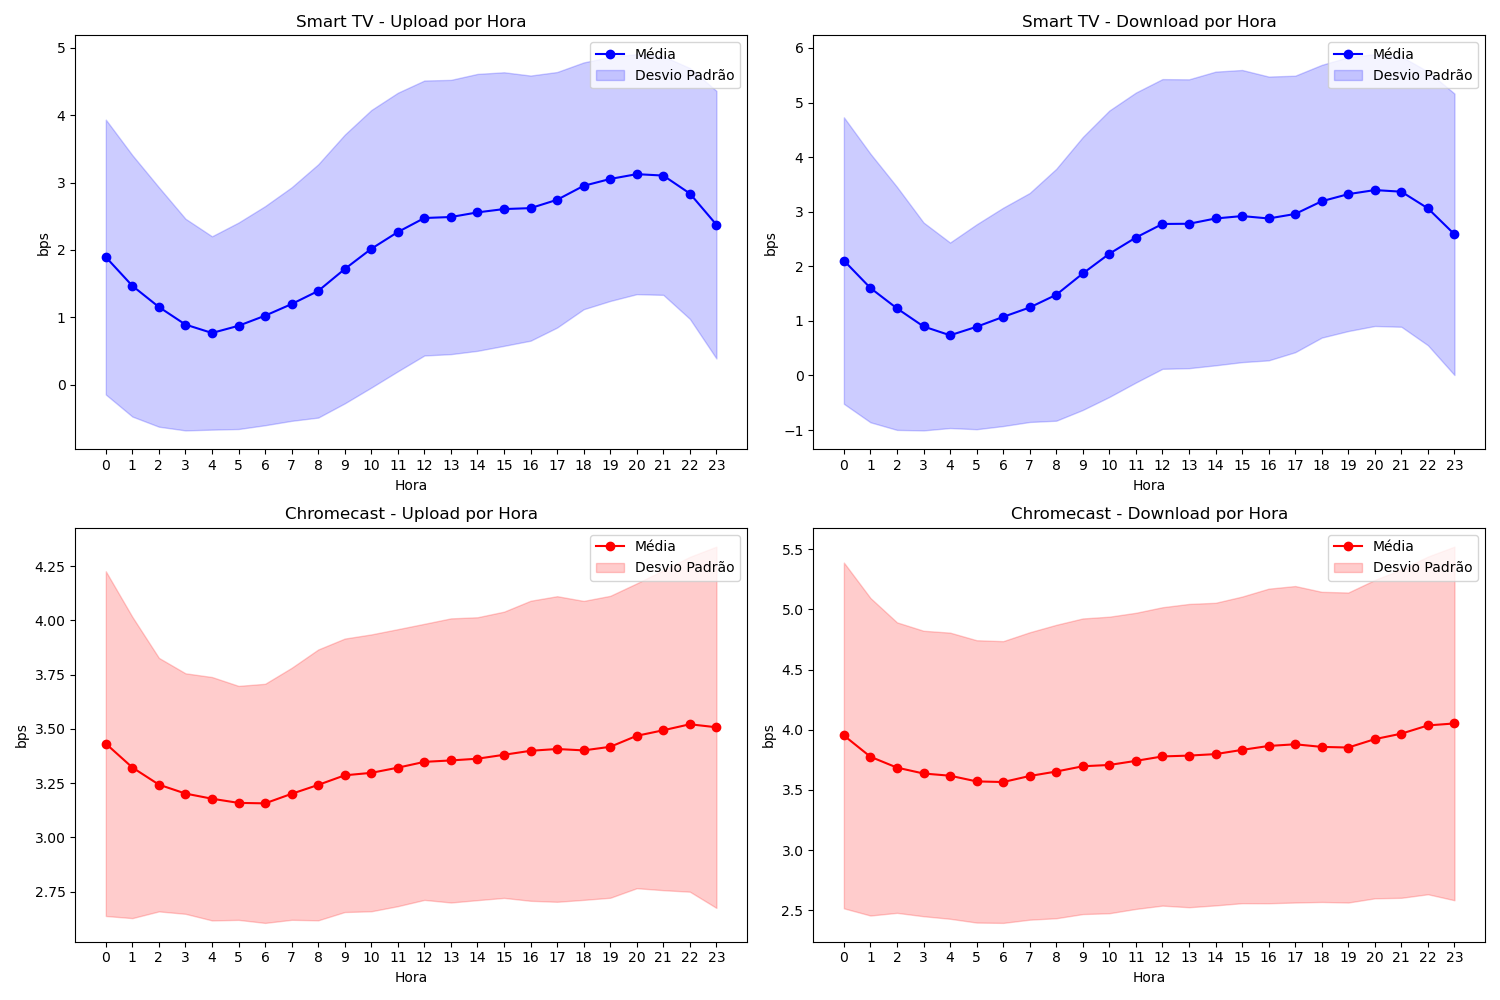
\includegraphics[width=0.8\textwidth]{../estatísticas por hora/estatisticas_por_hora.png}
    \caption{Gráficos das estatísticas por horário para Smart TV e Chromecast}
    \label{fig:estatisticas_por_hora}
\end{figure}

Além disso, foram gerados boxplots para cada hora do dia, separados por tipo de dispositivo e tipo de tráfego. As Figuras \ref{fig:boxplot_smart_up} e \ref{fig:boxplot_smart_down} exibem os boxplots das taxas de upload e download para o dispositivo Smart TV, respectivamente. Já as Figuras \ref{fig:boxplot_chrome_up} e \ref{fig:boxplot_chrome_down} mostram os boxplots das taxas de upload e download para o dispositivo Chromecast, respectivamente.

\begin{figure}[H]
    \centering
    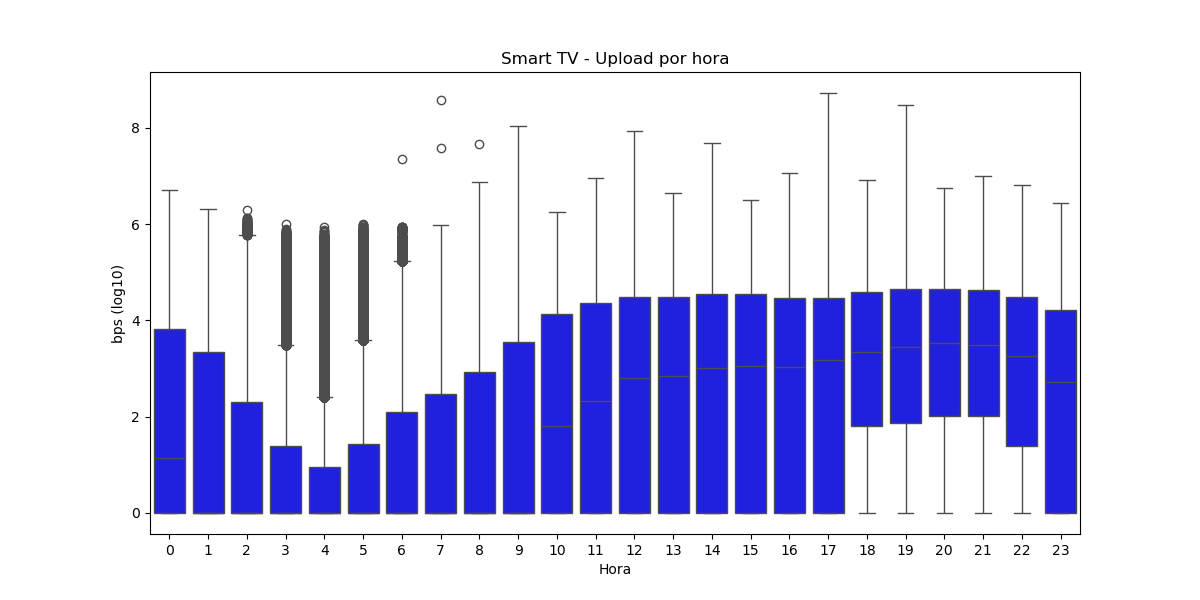
\includegraphics[width=0.8\textwidth]{../estatísticas por hora/boxplot_smart_up.png}
    \caption{Boxplot das taxas de upload para Smart TV}
    \label{fig:boxplot_smart_up}
\end{figure}

\begin{figure}[H]
    \centering
    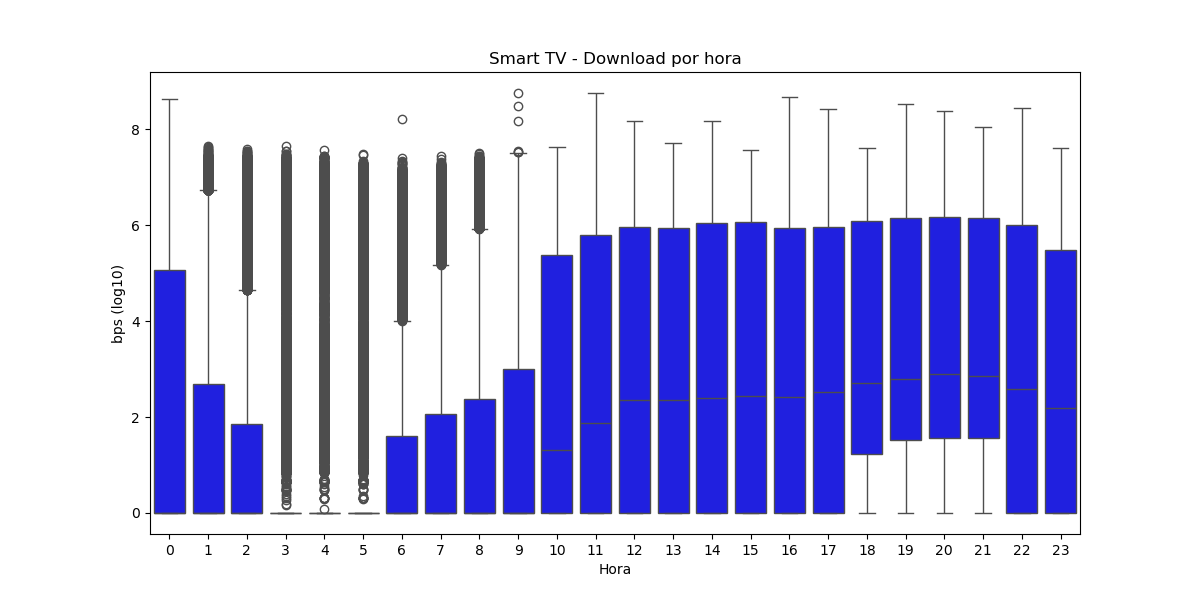
\includegraphics[width=0.8\textwidth]{../estatísticas por hora/boxplot_smart_down.png}
    \caption{Boxplot das taxas de download para Smart TV}
    \label{fig:boxplot_smart_down}
\end{figure}

\begin{figure}[H]
    \centering
    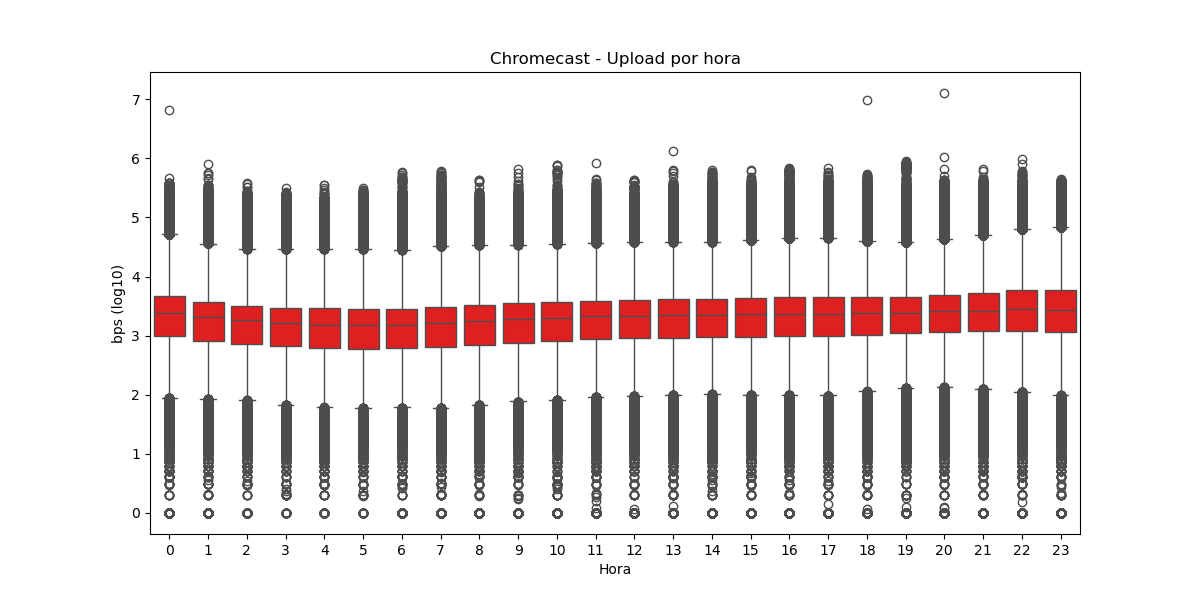
\includegraphics[width=0.8\textwidth]{../estatísticas por hora/boxplot_chrome_up.png}
    \caption{Boxplot das taxas de upload para Chromecast}
    \label{fig:boxplot_chrome_up}
\end{figure}

\begin{figure}[H]
    \centering
    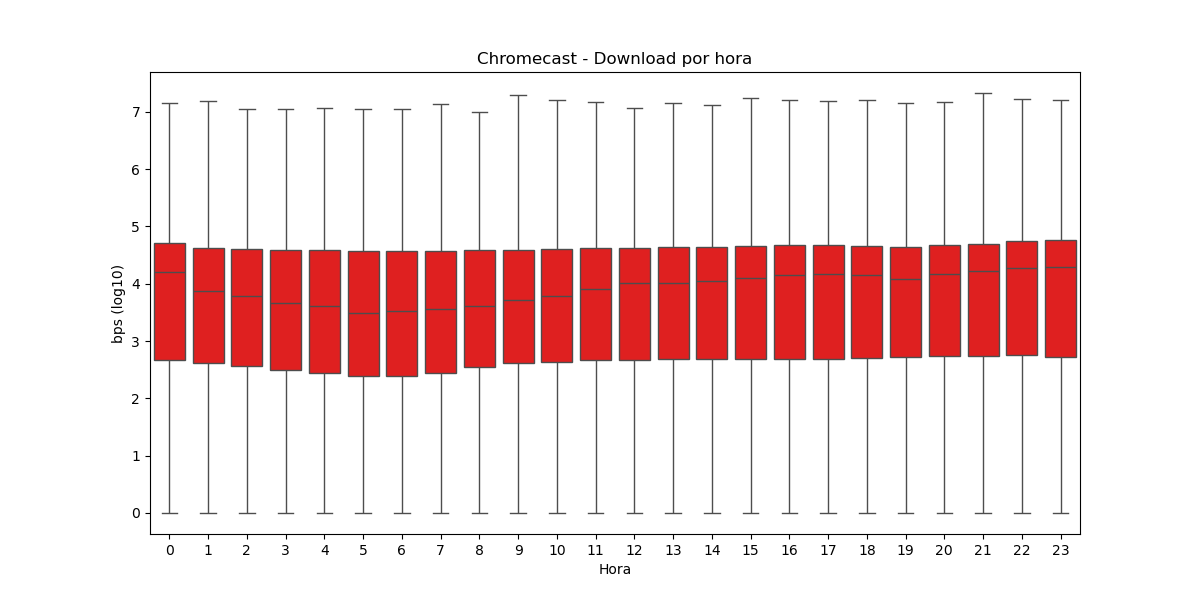
\includegraphics[width=0.8\textwidth]{../estatísticas por hora/boxplot_chrome_down.png}
    \caption{Boxplot das taxas de download para Chromecast}
    \label{fig:boxplot_chrome_down}
\end{figure}

\subsection{Análise dos Resultados}
\label{sec:analise_resultados_horario}

A partir da Tabela \ref{tab:estatisticas_por_horario} (e, consequentemente, da Figura  \ref{fig:estatisticas_por_hora}) e dos boxplots das figuras~\ref{fig:boxplot_smart_up}, \ref{fig:boxplot_smart_down}, \ref{fig:boxplot_chrome_up} e \ref{fig:boxplot_chrome_down}, podemos tirar algumas conclusões importantes sobre o comportamento das taxas de upload e download para os dispositivos Smart TV e Chromecast ao longo das 24 horas do dia:

\begin{itemize}
    \item \textbf{Smart TV:}
    \begin{itemize}
        \item As taxas de download e upload variam ao longo do dia, com uma tendência de aumento nas horas da tarde e noite.
        \item A média das taxas de download e upload é geralmente menor durante a madrugada e aumenta gradualmente até atingir picos durante a noite (20h tanto para download quanto para upload).
    \end{itemize}
    \item \textbf{Chromecast:}
    \begin{itemize}
        \item As taxas de download e upload para o Chromecast são consistentemente mais altas do que para a Smart TV, especialmente durante as horas da tarde e noite.
        \item A média das taxas de download e upload é relativamente estável ao longo do dia, em comparação com a Smart TV.
        \item Os picos de média ocorrem durante a noite (23h para download e 22h para upload), indicando um uso mais intenso da rede nesses horários.
        \item A variância e o desvio padrão das taxas de download e upload são menores para o Chromecast, indicando uma utilização mais consistente da rede.
    \end{itemize}
\end{itemize}

Essas observações sugerem que o uso da rede para a Smart TV é mais variável e depende mais do horário do dia, enquanto o Chromecast apresenta um uso mais constante. Isso pode ser devido a diferentes padrões de uso dos dispositivos, onde a Smart TV pode ser mais utilizada para atividades que demandam maior largura de banda em horários específicos, como streaming de vídeos em alta definição durante a tarde e noite.



\section{Caracterizando os Horários com Maior Valor de Tráfego}

Nesta seção, os horários com maior valor médio das taxas de upload e download para cada tipo de dispositivo, Smart TV e Chromecast, foram analisados seguindo os passos descritos.

\subsection{Passo 1: Seleção dos Horários}

A partir dos gráficos de médias por hora apresentados Figura~\ref{fig:estatisticas_por_hora}, os horários com maior valor médio para cada taxa e dispositivo foram identificados:
\begin{itemize}
    \item \textbf{Smart TV:}
        \begin{itemize}
            \item dataset 1: composto pelo horário com maior média de upload (20:00).
            \item dataset 2: composto pelo horário com maior média de download (20:00).
        \end{itemize}
    \item \textbf{Chromecast:}
        \begin{itemize}
            \item dataset 3: composto pelo horário com maior média de upload (22:00).
            \item dataset 4: composto pelo horário com maior média de download (23:00).
        \end{itemize}
\end{itemize}

\subsection{Passo 2: Histogramas dos Dados}

Histogramas foram gerados para cada um dos 4 datasets criados no Passo 1. O método de Sturges (Equação~\ref{eq:sturges}) foi utilizado para determinar o número adequado de bins, obtendo-se os seguintes valores:

\begin{itemize}
    \item \textbf{Dataset 1}(Smart TV - Upload)\textbf{:}  19 bins
    \item \textbf{Dataset 2}(Smart TV - Download)\textbf{:}  19 bins
    \item \textbf{Dataset 3}(Chromecast - Upload)\textbf{:}  20 bins
    \item \textbf{Dataset 4}(Chromecast - Download)\textbf{:}  20 bins
\end{itemize}

Esses histogramas destacam os padrões de distribuição das taxas de upload e download para os horários selecionados, conforme ilustrado na Figura~\ref{fig:histogramas_horarios}.

\begin{figure}[H]
    \centering
    \includegraphics[width=0.8\textwidth]{../caracterizando os horários/histogramas.png}
    \caption{Histogramas das taxas de upload e download para os horários selecionados.}
    \label{fig:histogramas_horarios}
\end{figure}

\subsection{Passo 3: Estimativa de Parâmetros via MLE}

Os parâmetros das distribuições Gaussiana e Gamma foram estimados utilizando o método de Máxima Verossimilhança (\textit{Maximum Likelihood Estimation} - MLE) para os quatro conjuntos de dados. Esses valores foram aplicados na modelagem das distribuições, permitindo uma análise comparativa com os dados observados.

O MLE consiste em determinar os parâmetros que maximizam a função de verossimilhança, que mede a probabilidade dos dados observados para um conjunto de parâmetros. Para simplificar os cálculos, o logaritmo da verossimilhança (\textit{log-likelihood}) é utilizado. A derivada da \textit{log-likelihood} é igualada a zero para encontrar os estimadores de máxima verossimilhança dos parâmetros.

As funções de densidade de probabilidade para as distribuições Gaussiana e Gamma são definidas como:

\begin{itemize}
    \item \textbf{Gaussiana:}
    \begin{equation}
        f(x) = \frac{1}{\sigma \sqrt{2\pi}} e^{-\frac{(x - \mu)^2}{2\sigma^2}}
    \end{equation}
    onde \(\mu\) é a média e \(\sigma^2\) é a variância da distribuição.
    
    \item \textbf{Gamma:}
    \begin{equation}
        f(x) = \frac{\beta^\alpha x^{\alpha - 1} e^{-x/\beta}}{\Gamma(\alpha)}
    \end{equation}
    onde \(\alpha\) é o parâmetro de forma, \(\beta\) é o parâmetro de escala, e \(\Gamma(\alpha)\) é a função Gamma, definida como \(\int_0^\infty x^{\alpha - 1} e^{-x} dx\).
\end{itemize}

Para a distribuição Gaussiana, as estimativas dos parâmetros são obtidas de forma direta:

\begin{equation}
    \hat{\mu} = \frac{1}{n} \sum_{i=1}^{n} x_i, \quad \hat{\sigma}^2 = \frac{1}{n} \sum_{i=1}^{n} (x_i - \hat{\mu})^2
\end{equation}

No caso da distribuição Gamma, a estimação dos parâmetros \(\alpha\) (forma) e \(\beta\) (escala) pelo MLE não possui soluções analíticas simples e geralmente requer métodos numéricos iterativos. O parâmetro \(\alpha\) é frequentemente estimado utilizando o método de Newton-Raphson aplicado à função de log-verossimilhança, enquanto \(\beta\) pode ser estimado a partir de \(\alpha\) e da média amostral \(\bar{x}\) \cite{minka2002estimating}:

\begin{equation}
    \hat{\beta} = \frac{\bar{x}}{\hat{\alpha}}
\end{equation}

Para realizar essas estimativas, foi utilizado o método \texttt{gamma.fit} da biblioteca \texttt{scipy.stats} do Python. Este método aplica o MLE de forma eficiente, empregando algoritmos de otimização numérica para determinar os parâmetros que melhor se ajustam aos dados observados. Além dos parâmetros de forma (\(\alpha\)) e escala (\(\beta\)), o método também estima o parâmetro de localização (\(loc\)), que desloca a distribuição Gamma ao longo do eixo \(x\). Esse deslocamento é essencial quando os dados incluem valores iguais a zero (o que é o caso, como mostrado na Seção~\ref{sec:eda}), já que a função de densidade de probabilidade (PDF) da distribuição Gamma é indefinida para \(x = 0\) quando \(loc = 0\). Com \(loc > 0\), a PDF é modificada para começar em \(x = loc\), tornando possível ajustar a distribuição mesmo em presença de valores nulos ou muito baixos. A utilização desse parâmetro garante que a modelagem estatística permaneça válida e consistente com as características dos dados.


Os resultados das estimativas de parâmetros via MLE para as distribuições Gaussiana e Gamma são apresentados na Tabela~\ref{tab:resultados_mle}.

\begin{table}[H]
    \centering
    \caption{Resultados das estimativas de parâmetros via MLE}
    \label{tab:resultados_mle}
    \begin{tabular}{|c|c|c|c|c|c|}
        \hline
        \textbf{Dataset} & $\boldsymbol{\hat{\mu}}$ & $\boldsymbol{\hat{\sigma}^2}$ & $\boldsymbol{\hat{\alpha}}$ & $\boldsymbol{\hat{\beta}}$ & $\boldsymbol{\textit{loc}}$ \\ 
        \hline
        Dataset 1 (Smart TV - Upload) & 3.2243 & 3.1687 & 214.6171 & 0.1245 & -23.4982 \\ 
        \hline
        Dataset 2 (Smart TV - Download) & 3.4961 & 6.2013 & 883.8791 & 0.0838 & -70.5760 \\ 
        \hline
        Dataset 3 (Chromecast - Upload) & 3.6215 & 0.5957 & 3078.6394 & 0.0139 & -39.2307 \\ 
        \hline
        Dataset 4 (Chromecast - Download) & 4.1527 & 2.1594 & 27.1301 & 0.2832 & -3.5314 \\ 
        \hline
        \end{tabular}
    \end{table}

    Além disso, as \textit{log-likelihoods} e \textit{likelihoods} para as distribuições Gaussiana e Gamma são apresentadas na Tabela~\ref{tab:likelihoods}. As \textit{log-likelihoods} foram calculadas primeiro, para evitar erros de \textit{underflow} ao calcular as \textit{likelihoods}, substituindo a multiplicação de valores muito pequenos pela soma de seus logaritmos naturais.
    \begin{table}[H]
        \centering
        \caption{Likelihoods ($L$) e Log-likelihoods ($\log[L]$) para os Datasets}
        \label{tab:likelihoods}
        \begin{adjustbox}{center}
        \begin{tabular}{|c|c|c|c|c|}
        \hline
        \textbf{Dataset} & $\boldsymbol{\log[L]}$ \textbf{Gaussiana} & $\boldsymbol{L}$ \textbf{Gaussiana} & $\boldsymbol{\log[L]}$ \textbf{Gamma} & $\boldsymbol{L}$ \textbf{Gamma} \\ 
        \hline
        Dataset 1 (Smart TV - Upload) & -424282 & 0 & -427222 & 0 \\ 
        \hline
        Dataset 2 (Smart TV - Download) & -495658 & 0 & -495518 & 0 \\ 
        \hline
        Dataset 3 (Chromecast - Upload) & -89011 & 0 & -89015 & 0 \\ 
        \hline
        Dataset 4 (Chromecast - Download) & -129603 & 0 & -128993 & 0 \\ 
        \hline
        \end{tabular}
        \end{adjustbox}
    \end{table}

Os valores nulos das \textit{likelihoods} indicam que as distribuições propostas (Gaussiana e Gamma) não são adequadas para modelar os dados observados. Isso será visualizado melhor na próxima seção, onde os histogramas dos dados e as funções de densidade parametrizadas serão comparados.

\subsection{Passo 4: Gráficos de Densidade}

Gráficos contendo o histograma dos dados e as funções de densidade Gaussiana e Gamma, parametrizadas pelos valores obtidos no Passo 3, foram gerados utilizando o método \texttt{pdf} das classes \texttt{scipy.stats.norm} e \texttt{scipy.stats.gamma} do Python. Esses gráficos permitem uma comparação visual da aderência de cada distribuição aos dados reais e estão disponíveis na Figura~\ref{fig:histogramas_pdf}.

\begin{figure}[H]
    \centering
    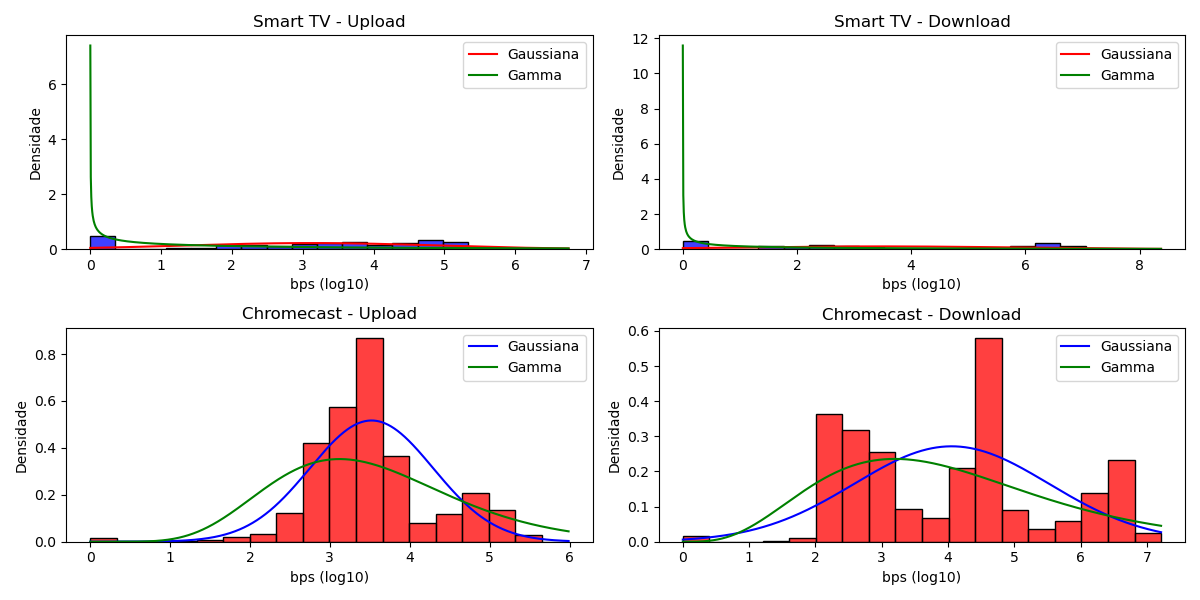
\includegraphics[width=0.8\textwidth]{../caracterizando os horários/histogramas_pdf.png}
    \caption{Histogramas dos dados e funções de densidade parametrizadas para as distribuições Gaussiana e Gamma.}
    \label{fig:histogramas_pdf}
\end{figure}

Observando a figura, é possível notar que nenhuma das distribuições propostas (Gaussiana e Gamma) se ajusta bem aos dados observados. Os histogramas sugerem que os dados não seguem uma distribuição normal e nem gamma, o que pode ser um dos motivos para a má aderência das distribuições propostas. A tabela de \textit{likelihoods} também indica que as distribuições propostas não são adequadas para modelar os dados, já que as \textit{log-likelihoods} são muito negativas, acarretando em \textit{likelihoods} nulas.

Uma sugestão seria utilizar uma mistura de distribuições para representar os dados, da seguinte forma:

\begin{itemize}
    \item \textbf{Dataset 1 (Smart TV - Upload):} Mistura de uma Gaussiana e uma Gamma.
    \item \textbf{Dataset 2 (Smart TV - Download):} Mistura de três Gaussianas.
    \item \textbf{Dataset 3 (Chromecast - Upload):} Mistura de duas Gaussianas.
    \item \textbf{Dataset 4 (Chromecast - Download):} Mistura de uma Gaussiana e duas Gammas.
\end{itemize}

Outra abordagem seria estimar a distribuição empírica dos dados, sem a necessidade de assumir uma distribuição paramétrica específica. Isso poderia ser feito utilizando métodos não paramétricos, como o estimador de densidade de Kernel (em inglês, \textit{Kernel Density Estimator} - KDE), que não requer a especificação de uma forma funcional para a distribuição dos dados. Utilizando o parametro KDE da biblioteca \texttt{seaborn} do Python, é possível estimar a distribuição empírica dos dados, como mostrado na Figura~\ref{fig:histogramas_pdf_kde}.

\begin{figure}[H]
    \centering
    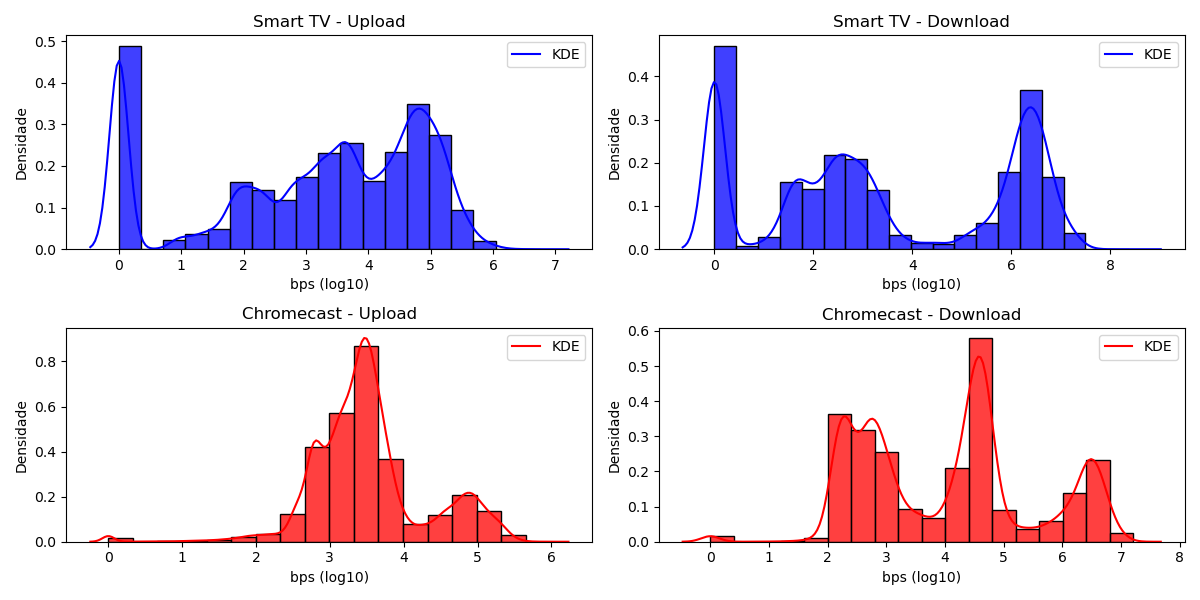
\includegraphics[width=0.8\textwidth]{../caracterizando os horários/histogramas_pdf_kde.png}
    \caption{Histogramas dos dados e estimativas de densidade empírica utilizando KDE.}
    \label{fig:histogramas_pdf_kde}
\end{figure}

\subsection{Passo 5: Probability Plots}

\textit{Probability Plots} foram criados para comparar os dados reais com as distribuições parametrizadas (Gaussiana e Gamma), utilizando o método \texttt{probplot} da biblioteca \texttt{scipy.stats} do Python.

No total, 8 gráficos foram gerados, permitindo avaliar a adequação das distribuições propostas aos dados. Essas gráficos podem ser observados nas Figuras~\ref{fig:probplot_gaussiana} e~\ref{fig:probplot_gamma}.

\begin{figure}[H]
    \centering
    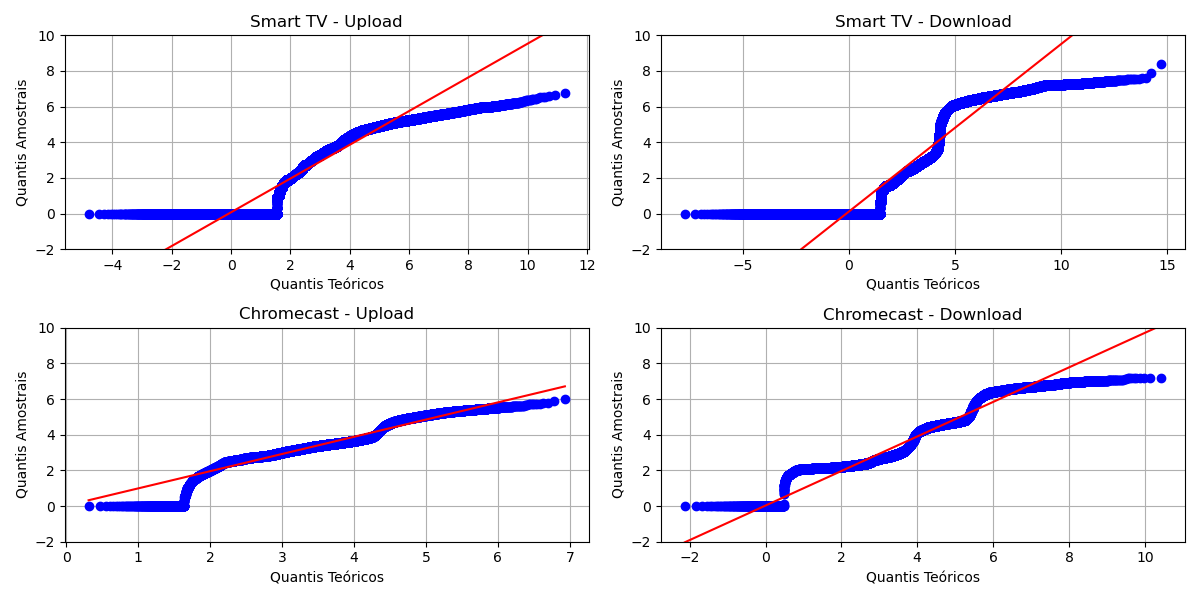
\includegraphics[width=0.8\textwidth]{../caracterizando os horários/probplot_gaussiana.png}
    \caption{Probability Plots para as distribuições Gaussiana.}
    \label{fig:probplot_gaussiana}
\end{figure}

\begin{figure}[H]
    \centering
    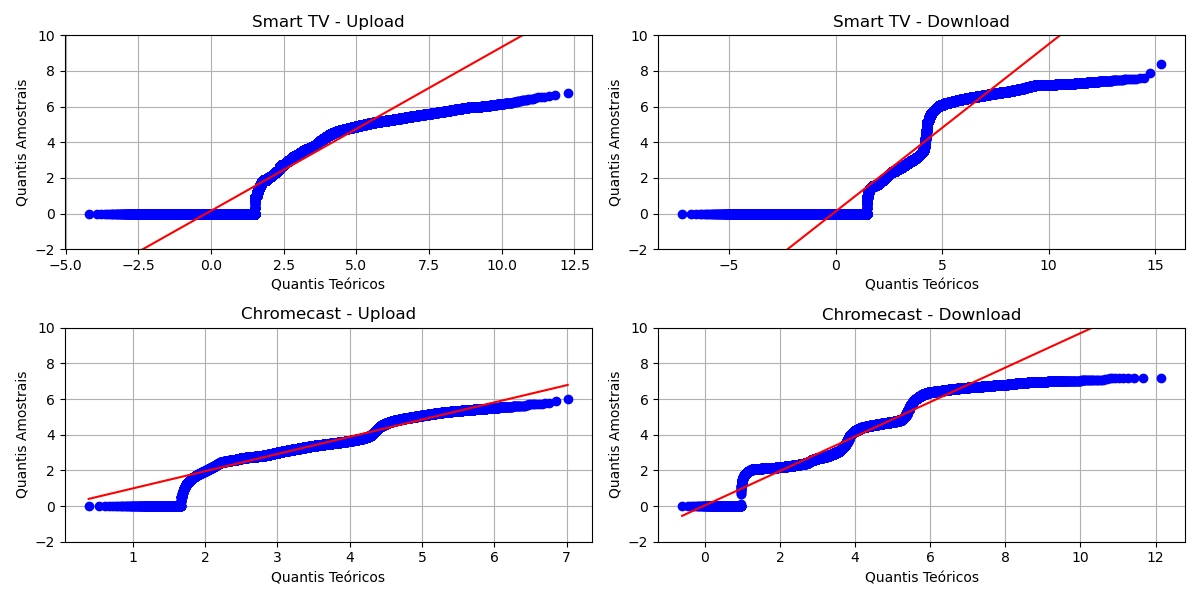
\includegraphics[width=0.8\textwidth]{../caracterizando os horários/probplot_gamma.png}
    \caption{Probability Plots para as distribuições Gamma.}
    \label{fig:probplot_gamma}
\end{figure}

A avaliação dos \textit{probability plots} revela que a distribuição Gaussiana apresenta um ajuste insatisfatório para todos os datasets analisados. Em todos os casos, observa-se que os pontos se distanciam consideravelmente da linha reta nas regiões extremas, com aproximação parcial na região central. No entanto, mesmo nessa aproximação, os pontos oscilam de forma significativa em torno da linha, indicando inconsistências no ajuste. A Gaussiana não consegue capturar a assimetria dos dados nem modelar adequadamente a alta concentração de valores baixos ou iguais a zero, como observado nas taxas de upload e download da Smart TV e do Chromecast.

A distribuição Gamma, apesar de ser mais flexível, também apresentou resultados insatisfatórios. Assim como a Gaussiana, os \textit{probability plots} mostram que a Gamma se distancia excessivamente da linha reta nos valores extremos e, embora se aproxime dela nos valores centrais, essa aproximação é marcada por oscilações significativas. Mesmo com o uso do parâmetro de deslocamento (\(loc\)) para lidar com os valores nulos, a distribuição Gamma não foi capaz de capturar a alta densidade de valores próximos de zero nem os padrões de dispersão observados. Dessa forma, ambas as distribuições falham em modelar adequadamente os dados analisados.
adequada que a Gaussiana para os dados analisados.

\subsection{Passo 6: QQ Plots}

Foram gerados \textit{QQ Plots} para comparar os dados de upload e download entre os dispositivos Smart TV e Chromecast, considerando os horários de maior tráfego identificados nos passos anteriores. Os conjuntos de dados da Smart TV (\textit{datasets} 1 e 3) são os maiores, enquanto os do Chromecast (\textit{datasets} 2 e 4) são os menores. A interpolação foi implementada utilizando a função \texttt{numpy.interp}, que aplica a seguinte fórmula básica de interpolação linear:
\[
y = y_1 + \frac{(x - x_1)(y_2 - y_1)}{(x_2 - x_1)},
\]
onde \(x\) representa os quantis do menor conjunto de dados (Chromecast), \(x_1\) e \(x_2\) são quantis do maior conjunto (Smart TV) que cercam \(x\), e \(y_1\) e \(y_2\) são os valores correspondentes no maior conjunto. Esse procedimento garante que os quantis dos dois conjuntos sejam comparados de forma consistente, ajustando o conjunto maior (Smart TV) para alinhar-se ao conjunto menor (Chromecast).

Os \textit{QQ Plots} comparando as taxas de upload dos dispositivos Smart TV (\textit{dataset} 1) e Chromecast (\textit{dataset} 3), e as taxas de download dos dispositivos Smart TV (\textit{dataset} 2) e Chromecast (\textit{dataset} 4) são apresentados na Figura~\ref{fig:qq_plot}.

\begin{figure}[H]
    \centering
    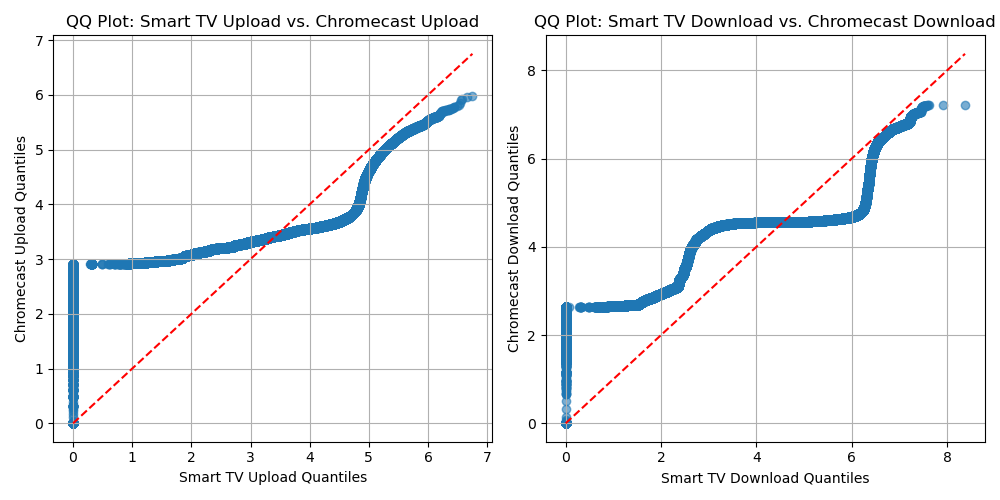
\includegraphics[width=0.8\textwidth]{../caracterizando os horários/qq_plot.png}
    \caption{QQ Plots para os horários de maior tráfego dos dispositivos Smart TV e Chromecast.}
    \label{fig:qq_plot}
\end{figure}

Os \textit{QQ Plots} indicam diferenças marcantes entre os padrões de tráfego da Smart TV e do Chromecast para upload e download. Na região inicial, observa-se uma linha horizontal paralela ao eixo dos quantis do Chromecast, indicando que, enquanto a Smart TV possui muitos valores nulos (\(x = 0\)), Chromecast apresenta valores positivos não nulos. Esse comportamento reflete uma discrepância significativa na forma como os dois dispositivos tratam os valores iniciais.

Na região central dos gráficos, os pontos continuam desalinhados em relação à linha de referência (\(y = x\)), evidenciando que as distribuições dos dois dispositivos possuem padrões distintos. A variabilidade na Smart TV é mais ampla, o que contribui para a diferença estrutural entre os conjuntos. Esse desalinhamento é consistente tanto para upload quanto para download.

Nas caudas superiores, os pontos mostram que os valores da Smart TV são significativamente maiores do que os do Chromecast. Isso sugere que a Smart TV possui uma maior proporção de valores extremos, indicando uma maior variabilidade e dispersão dos dados. Essa diferença é mais acentuada para o download, onde a Smart TV apresenta valores mais altos do que o Chromecast.

\subsection{Análise dos Resultados}

Com base nos resultados, as seguintes questões foram avaliadas:
\begin{enumerate}
    \item \textbf{Quais foram os horários escolhidos para cada dataset?}
    \item \textbf{O que foi observado a partir dos histogramas?}
    \item \textbf{Quais diferenças e/ou similaridades foram identificadas entre os datasets 1, 2, 3 e 4?}
    \item \textbf{É possível caracterizar os datasets por uma variável aleatória conhecida na literatura? Se não, por quê?}
    \item \textbf{O que foi observado a partir dos gráficos \textit{QQ Plot} e \textit{Probability Plot}?}
\end{enumerate}
% As conclusões são apresentadas em termos de suas implicações para o gerenciamento da rede e o entendimento dos padrões de tráfego para Smart TVs e Chromecasts.


\section{Códigos}

Os códigos utilizados em todas as etapas deste projeto estão disponíveis no repositório do GitHub: \url{https://github.com/lhscaldas/Projeto_Probabilidade_e_Estatistica}

\bibliographystyle{abntex2-num} % Escolha o estilo de citação desejado
\nocite{Kobayashi_2011}
\nocite{Pishro_2014}
\bibliography{bibliografia} % Nome do arquivo .bib (sem a extensão)

\end{document}